\section{Fluid Dynamics}
The aim of Computational fluid dynamics is to approximate numerically the physical conservation laws of newtonian physics:

\begin{itemize}
  \item conservation of mass

  \item The conservation of momentum (Newton’s second law, the rate of change of momentum equals the sum of forces acting on the fluid);

  \item The conservation of energy (first law of thermodynamics, the rate of change of energy equals the sum of rate of heat addition to and the rate of work done on the fluid).

\end{itemize}

    \subsection{Mass Conservation}

    The principle of conservation of mass is that, in a closed system, the mass remains constant. This means that fluid will move through a set region in such a way the mass is conserved. For an incompressible flow, this means that the outflows and the inflows will be equal. This can be written as
    \begin{equation} \label{eq:1}
      0 = \sum_{in} \dot{m} - \sum_{out} \dot{m}
    \end{equation} 

    Where $\dot{m}$ = mass flow rate.
    
    The mass flow rate can be written as $ \rho u A $,  for $\rho$ = density, $u$ = velocity and A is the scross sectional area of the flow. For flow in the x direction, $ A = \Delta z \Delta x $. For a two dimensional flow, $ \Delta z = 1 $, giving:

    \begin{equation} \label{eq:2}
      \dot{m}_{in} = \rho u \Delta y
    \end{equation}

    Extending this to equation \ref{eq:1}, in the x direction, for an incompressible flow we get

    \begin{equation} \label{eq:3}
      0 = \rho u_{in} \Delta y_{in} - \rho u_{out} \Delta y_{out}
    \end{equation}

    This can easily be extrapolated to three dimensions.
\begin{figure}   
  \centering
  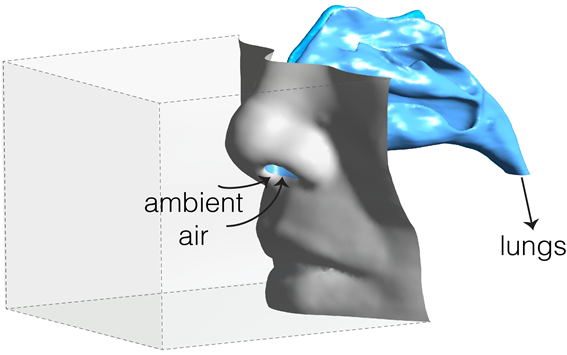
\includegraphics[width=0.5\textwidth]{CompDom}
  \caption{Fluid moving through the computational domain, the inflow of ambient air must be equal to the air entering the lungs}
  \label{fig:CompDom}
\end{figure}
    In the case of the nasal cavity, this can be conceptualised in relation to the nasal cavity geometry, where the air flow rate going in to the nostrils must be equal to that leaving through the extension from the nasopharynx, as seen in figure \ref{fig:CompDom}.



    \subsection{Momentum Conservation}

    Momentum conservation is based on the Newton's second law:

    \centerline{$\sum F = ma$}

    Here $m$ is the mass of the system, $a$ is its rate of acceleration, and  $\sum F$ is the sum of forces acting on the system. F can generally be divided in to body and surface forces. Rewriting the mass as the product of volume and the density, and acceleration as the first derivative of velocity:


    \begin{equation} \label{eq:4}
      \sum F_{body} + \sum F_{surface} = (\rho \Delta x \Delta y \Delta Z) \frac{DU}{Dt}
    \end{equation}

    Body forces generally include gravity, centrifugal, Coriolis and electromagnetic forces; these all act on the volume from a distance.

    Surface forces are those that act directly on the surface of a fluid element. These fluid forces include normal stress, in the x direction $\sigma_{xx}$, which is made up of pressure forces $p$ exerted on the body and normal viscous stress components $tau_{xx}$; and tangential stresses, $\tau_{xy}$ and $\tau_{xz}$.

    Summing these forces in the x direction, for a 2D fluid element we get:
    

    \begin{dmath} \label{eq:5}
      \sum F_{surface, x} = [\sigma_{xx} \Delta y \Delta z - (\frac{\delta \sigma_{xx}}{\delta x} \Delta x) \Delta y \Delta z] 
      + [(\tau_{xy} + \frac{\delta \tau_{yx}}{\delta y} \Delta y) \Delta x \Delta z - \tau_{yx} \Delta x \Delta z]  
      = - \frac{\delta \sigma_{xx}}{\delta x} \Delta x \Delta y \Delta z + \frac{\delta \tau_{yx}}{\delta y} \Delta x \Delta y \Delta z
    \end{dmath}


    Assuming that the fluid is Newtonian and isotropic, $\sigma_{xx}$ can be related to pressure $p$ and viscous stresses $\tau_{xx}$ by

    \centerline{$\sigma_{xx} = -p + \tau_{xx}$}

    For a Newtonian fluid, stress-strain relations can be described as 

    \begin{equation} \label{eq:6}
      \tau_{xx} = 2 \mu \frac{\delta u}{\delta x} \quad \tau_{yx} = \mu \frac{\delta u}{\delta y}
    \end{equation}

    Where $\mu$ is the viscocity of the fluid. Combining equations \ref{eq:4} , \ref{eq:5} and \ref{eq:6} in the x direction, and cancelling out the volume term:

    \begin{equation} \label{eq:7}
      \rho \frac{Du}{Dt} = - \frac{\delta p}{\delta x} + \mu (\frac{\delta^2 u}{\delta x^2} + \frac{\delta^2 u}{\delta y^2}) + \rho \sum F_{b}
    \end{equation}
    
    Here the acceleration term is the total derivative of u, defined as the combined local and advection inertial forces, which in two dimensions can be written as

    \begin{equation} \label{eq:8}
      \frac{Du}{Dt} = \frac{\delta u}{\delta t} + v \frac{\delta u}{\delta y} + u \frac{\delta u}{\delta x}
    \end{equation}

    combining equations \ref{eq:7} and \ref{eq:8} and dividing through by $\rho$:

    \begin{equation} \label{eq:9}
      \underbrace{\frac{\delta u}{\delta t}}_{local\ acceleration} + v \underbrace{\frac{\delta u}{\delta y} + u \frac{\delta u}{\delta x}}_{convection} = - \underbrace{\frac{1}{\rho} \frac{\delta p}{\delta x}}_{pressure gradient} + \underbrace{\nu (\frac{\delta^2 u}{\delta x^2} + \frac{\delta^2 u}{\delta y^2})}_{diffusion} + \underbrace{\sum F_{b}}_{body force}
    \end{equation}

    Where $\nu$ is kinematic viscocity, defined as $\frac{\mu}{\rho}$. 

    \subsection{Energy Conservation}

    Conservation of energy is derived from the first law of thermodynamics, that in a steady flow system the total energy of a control volume remains constant; that inflows and outflows must be equal. This can be expressed analogously to the mass conservation as 

    \begin{equation} \label{eq:10}
      \frac{DE}{Dt} = \sum{\dot{Q}} + \sum{\dot{W}}
    \end{equation}

    Where $\dot{Q}$ is heat transfer and $\dot{W}$ is the rate of work done. $E$ is energy per unit mass and is expressed as

    \centerline{$E = C_{p} T$}

    $\frac{DE}{Dt}$ can be expressed similarly to Equation \ref{eq:8}:

    \begin{equation} \label{eq:11}
      \frac{DE}{Dt} = \frac{\delta E}{\delta t} + v \frac{\delta E}{\delta y} + u \frac{\delta E}{\delta x} = C_{p} (\frac{\delta T}{\delta t} + v \frac{\delta T}{\delta y} + u \frac{\delta T}{\delta x})
    \end{equation}

    For a 2D element, the total energy can therefore be calculated from

    \begin{equation} \label{eq:12}
      \rho \frac{DE}{Dt} \Delta x \Delta y = \rho   C_{p} (\frac{\delta T}{\delta t} + v \frac{\delta T}{\delta y} + u \frac{\delta T}{\delta x}) \Delta x \Delta y
    \end{equation}

    From Fourier's law of heat conduction, for a 2D system we can write

    \begin{equation} \label{eq:13}
      \dot{Q}_{x} = k A_{x} \frac{\delta T}{\delta x} = \dot{q}_{x} A_{x} = \dot{q}_{x} \Delta y
    \end{equation}

    where $\dot{q}$ is heat flux = $\dot{Q}/A$

    The heat transferred into the element can thus be expressed as

    \begin{equation} \label{eq:14}
      [q_{x} + \frac{\delta q_{x}}{\delta x}] \Delta y - q_{x} \Delta y = \frac{\delta q_{x}}{\delta x} = k \frac{\delta^2 T}{\delta x^2} \Delta x \Delta y
    \end{equation}

    \begin{figure} \label{fig:eneq}
      \caption{Flow of heat energy through a 2D element}
    \end{figure}

    reconstructing equation \ref{eq:10} with the inclusion of \ref{eq:14}, considered also in the y direction, we can cancel out the volume term:

    \begin{equation} \label{eq:15}
      \underbrace{\frac{\delta T}{\delta t}}_{local\ acceleration} + \underbrace{u \frac{\delta T}{\delta x} + v \frac{\delta T}{\delta y}}_{convection} = \underbrace{\frac{k}{\rho C_{p}} ( \frac{\delta^2 T}{\delta x^2} + \frac{\delta^2 T}{\delta y^2} )}_{diffusion}
    \end{equation}

\section{Humidity}

One of the primary functions of the nasal cavity is the humidification of the incoming air in preparation for its interaction with the lungs. It therefore stands that any investigation into the fluid mechanisms of the nasal cavity would be incomplete without adressing the efficacy of this function. One simple but effective method for approximating humidification data in a computational domain is the use of the convection-diffusion equation.

Analogously to equations \ref{eq:15} and \ref{eq:9}, for a 2D element we can write

\begin{equation} \label{eq:16}
  \underbrace{\frac{\delta C_{H_{2} O}}{\delta t}}_{local acceleration} + \underbrace{u \frac{\delta C_{H_{2} O}}{\delta x} + v \frac{\delta C_{H_{2} O}}{\delta y}}_{convection} = \underbrace{D_{H_{2} O} ( \frac{\delta^2 C_{H_{2} O}}{\delta x^2} + \frac{\delta^2 C_{H_{2} O}}{\delta y^2} )}_{diffusion}
\end{equation} \nocite{Naftali1998}

Where $C_{H_{2} O}$ is the concentration of water vapour and $D_{H_{2} O}$ is the diffusivity of water in air.

\begin{figure} \label{fig:h2oel}
  \caption{water vapour moving through a 2D element}
\end{figure}

\section{Solving the Governing Equations}

The conservation equations outlined earlier in this chapter are nonlinear partial differential equations which, for complex domains such as the nasal cavity geometry, have no analytical solution; they must therefore be approximated algebraically and solved numerically.

\subsection{Discretisation}

Approximating, or discretising a system to make it numerically solvable can be done in many ways. One of the more common methods in modern solvers is the finite volume method, which can be applied to unstructured as well as structured meshes, making it particularly suited to complex geometries such as that of the nasal cavity.

The Finite Volume Method discretises the system into a series of volumes. The fluxes of relevant variables through the different faces of each element are then treated as a discrete system, which is able to be solved numerically.

\begin{figure}
  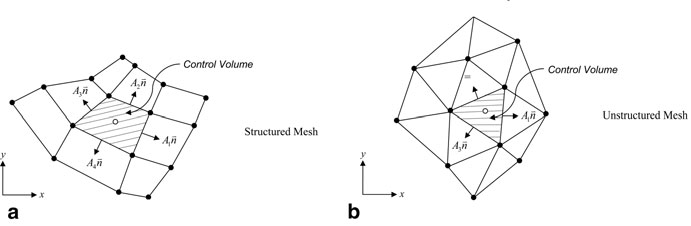
\includegraphics[width=\textwidth]{unstrfv}
  \caption{representation of mesh discretised with finite volume method}
  \label{usfv}
\end{figure}

Finite volume methods can tend to cause artificial, or numerical, diffusion if the mesh is of low quality. It is thus necessary to follow proper meshing practices, similar to those outlined in section \ref{Meshing}.

\subsection{Numerical Solution}

Once the system has been discretised, a system of linear equations can be developed to describe the system. These equations can be solved with one of several methods. These methods can generally be divided into two categories: either direct or iterative. In general, for large complex domains such as the nasal cavity models presented in this paper, iterative methods are the only way to derive a solution.

\section{Setup and Solution of Nasal Cavity Models Used in This Thesis}
Here an overview will be given of the way that the solution of the nasal cavity systems presented in this thesis will be given. Firstly the models are prepared and meshed as discussed in the chapter \ref{MRM}. Once this is done the boundary conditions for the system must be defined. 

The face and internal wall of the nasal cavity and pipe extension are set to no slip condition. This means that velocity is assumed to be zero on the surface of these zones. The exit of the pipe extension is given a constant velocity value calculated for each model as to give an inspiritory flow rate of 10 lpm, which has been suggested by the literature to be a realistic value for a resting flow rate. For these simulations this flow rate is treated as cunstant and the flow treated as steady, an assumption which greatly simplifies the solution process and one which is commonly used when comparing fluid flow characteristicsbetween nasal cavity models (transient, or time dependant solutions are computationally much more costly). 

The border of the hemispheric region around the face is set to atmospheric pressure. For resting inspiratory flow rates flows have been shown to be modeled most accurately as laminar; as such no turbulence model is used.

The numerical solution of the systems - described by the aforementioned boundary conitions and meshes - is approximated, for the models of this thesis, by the use of a commercial CFD code, in this case ANSYS FLUENT. The following chapter details the analysis of the solutions obtained for the five cavities.
